\documentclass[10pt,a4paper]{article}
\usepackage[latin1]{inputenc}
\usepackage{amsmath}
\usepackage{amsfonts}
\usepackage{amssymb}
\usepackage{fullpage}
\usepackage{graphicx}

\begin{document}
\title{J.D. Jackson Problem 11.6}
\author{Josh Orndorff \\ admin@joshorndorff.com}
\maketitle


The rocket's reference frame here is not inertial, which means that many of the transformations are not as straight-forward as usual.  In particular, $\gamma$ and $\beta$ are functions of time (either $t$ or $t'$).
\section{Velocity in the Earth's frame}
Although it is not asked for explicitly, I'll first find an expression for the rocket's velocity as measured in the Earth frame as a function of the rocket's proper time, $v(t')$. It may seem like a strange mixing of prime and unprime quantities, but this result will be useful a few times.

We'll use the results of problem 11.5  to see that
\begin{equation}
a=\frac{(1-\frac{v^2}{c^2})^{3/2}}{(1+\frac{v\cdot u}{c^2})^3} a'
\end{equation}
$u'=0$ because the rocket does not move in its own frame, so the entire denominator of the previous equation is one. Additionally, we know that $a'=g$ from the problem.
\begin{equation}
\frac{\mathrm{d}v}{\mathrm{d}t}=a=\left(1-\frac{v^2}{c^2}\right)^{3/2} g=\frac{g}{\gamma^3}
\end{equation}
\begin{equation}
\frac{\mathrm{d}v}{\mathrm{d}t}=\frac{\mathrm{d}v}{\gamma\mathrm{d}t'}
\end{equation}

We now have two expressions for $\frac{\mathrm{d}v}{\mathrm{d}t}$, so let's set them equal to each other.
\begin{equation}
\frac{\mathrm{d}v}{\gamma\mathrm{d}t'}=\frac{g}{\gamma^3}
\end{equation}

Cross multiplying, we have  $\gamma^2 \mathrm{d}v=g\,\mathrm{d}t'$, and we can integrate both sides
\begin{equation}
\int\frac{\mathrm{d}v}{\left(1-\frac{v(t')^2}{c^2}\right)}=\int g t'
\end{equation}
\begin{equation}
c \,\mathrm{arctanh}\left(\frac{v(t')}{c}\right)=gt'
\end{equation}
\begin{equation}\label{v/c of t'}
\frac{v(t')}{c}=\tanh\frac{gt'}{c}
\end{equation}
\begin{equation}\label{v of t'}
v(t')=c\tanh\frac{gt'}{c}
\end{equation}

\section{Travel time in Earth frame}
Having that preliminary result out of the way, we're now ready to solve for the required quantities.  We'll start by integrating the time dilation formula
\begin{equation}
\mathrm{d}t=\gamma \,\mathrm{d}t'
\end{equation}
\begin{equation}
\int\mathrm{d}t=\int\gamma \,\mathrm{d}t'
\end{equation}
\begin{equation} \label{time integral}
t=\int_0^{t'}\frac{\mathrm{d}t'}{\sqrt{1-\frac{v^2(t')}{c^2}}}
\end{equation}

Now we can refer back to our $v(t')$ expression (Eq: \ref{v/c of t'}).
\begin{equation}
t=\int_0^{t'}=\frac{\mathrm{d}t'}{\sqrt{1-\tanh^2\frac{gt'}{c}}}
\end{equation}
\begin{equation}\label{t of t'}\boxed{
t=\frac{c}{g}\sinh\frac{gt'}{c}
}\end{equation}

It is, perhaps, more insightful to write the previous equation as
\begin{equation}
\frac{gt}{c}=\sinh\frac{gt'}{c}
\end{equation}

Or, if we express both times as unitless quantities measured in multiples of $c/g$\footnote{Clocking in at 353.8 days, $c/g$ is remarkably close to one year. When $t'=5$ years, $\frac{gt'}{c}\approx 5$.}, then we can write $t=\sinh t'$.  We can see now that at launch, $t=t'=0$ the Earth's clock and the rocket's clock tick at the same speed.  But as the rocket continues to accelerate, it's clock apparently slows when observed from Earth.
\begin{figure}[h]
\centering
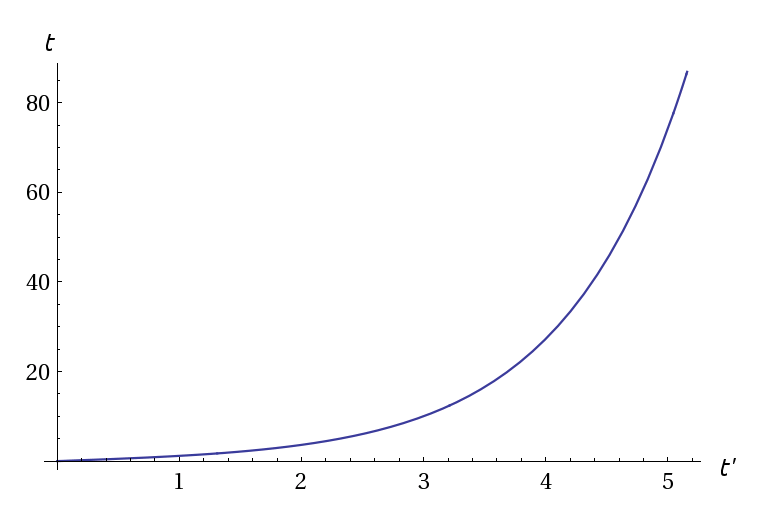
\includegraphics[scale=.4]{Jackson11-6-graph.png}
\caption{$t$ is related to $t'$ by a sinh function. Plot is in units pf $c/g$.}
\end{figure}

\section{Distance travelled in the Earth frame}

To find the distance travelled we will use the simplest kinematic equation.
\begin{equation}
d=vt
\end{equation}

We'll write the previous equation in differential form and use the chain rule
\begin{equation}
\mathrm{d}d=v(t')
\,\mathrm{d}t'\frac{\mathrm{d}t}{\mathrm{d}t'}
\end{equation}
\begin{equation}
d=\int v(t')\mathrm{d}t'\frac{\mathrm{d}t}{\mathrm{d}t'}
\end{equation}

We found $t$ as a function of $t'$, in Eq: \ref{t of t'}, so now we can differentiate it to write,
\begin{equation}
\frac{\mathrm{d}t}{\mathrm{d}t'}=\cosh\left(\frac{gt'}{c}\right)
\end{equation}

We will again use our result for $v(t')$ (this time in the form of Eq: \ref{v of t'}). So we can now find $d$.
\begin{equation}
d=\int_0^{t'} c \tanh\left(\frac{gt'}{c}\right)\mathrm{d}t' \cosh\left(\frac{gt'}{c}\right)
\end{equation}
\begin{equation}
d=c\int_0^{t'} \sinh\left(\frac{gt'}{c}\right)\mathrm{d}t'
\end{equation}
\begin{equation}
d=\frac{c^2}{g}\left[\cosh\left(\frac{gt'}{c}\right)\right]_0^{t'}
\end{equation}
\begin{equation}\boxed{
d=\frac{c^2}{g}\left[\cosh\left(\frac{gt'}{c}\right)-1\right]
}\end{equation}

\section{Some actual numbers}
The time for a quarter journey (a single acceleration) is given by
\begin{equation}
t_{1/4}=t(5 \,years)=84.24 \,years
\end{equation}
The total journey is four of these segments
\begin{equation}
T_{total}=4t_{1/4}=337 \,years
\end{equation}

Likewise, we can find the quarter journey distance
\begin{equation}
_{1/4}=d(5 \,years)=7.873 \times 10^{17} m
\end{equation}
\begin{equation}
d_{1/2}=2d_{1/4}=1.575\times 10^{18} m
\end{equation}

\end{document}